\chapter{simulation}\label{simulation}
\section{Geant4}
Geant4 とは物質中を通過する粒子の物理相互作用をモンテカルロ法に基づいてシミュレートすることのできるパッケージである.
物理プロセスや検出器の構造, 検出器の応答, 応答データ等の作成, 保存などの多くのツールキットから構成されている.

\section{本実験での$\mu$粒子シミュレーション}
宇宙線発生シミュレーションCRYを用いて$\mu$粒子を生成した.
装置のパラメーターは
\begin{quote}[H]
    \begin{itemize}
        \item トリガーシンチレータ126cm$\times$7cm$\times$1cmを7度ずつ傾けて横に3枚
        \item シンチレータ75cm$\times$4cm$\times$1cmを横に4枚, 縦に8層
        \item アルミニウム板100cm$\times$30cm$\times$2cmを8層
    \end{itemize}
\end{quote}
としてトリガーシンチレータのすぐ下からトリガーシンチレータの大きさの範囲で$10^{7}$イベントの$\mu$粒子を発生させた.
\\
CRYによって生成した$\mu$粒子のうち、
1番上のシンチレータに入射した粒子のエネルギー分布と角度分布がそれぞれ図\ref{fig:muon_energy_distribution}、図\ref{fig:muon_degree_distribution}である。
\begin{figure}[H]
    \begin{minipage}[b]{0.47\linewidth}
        \centering
        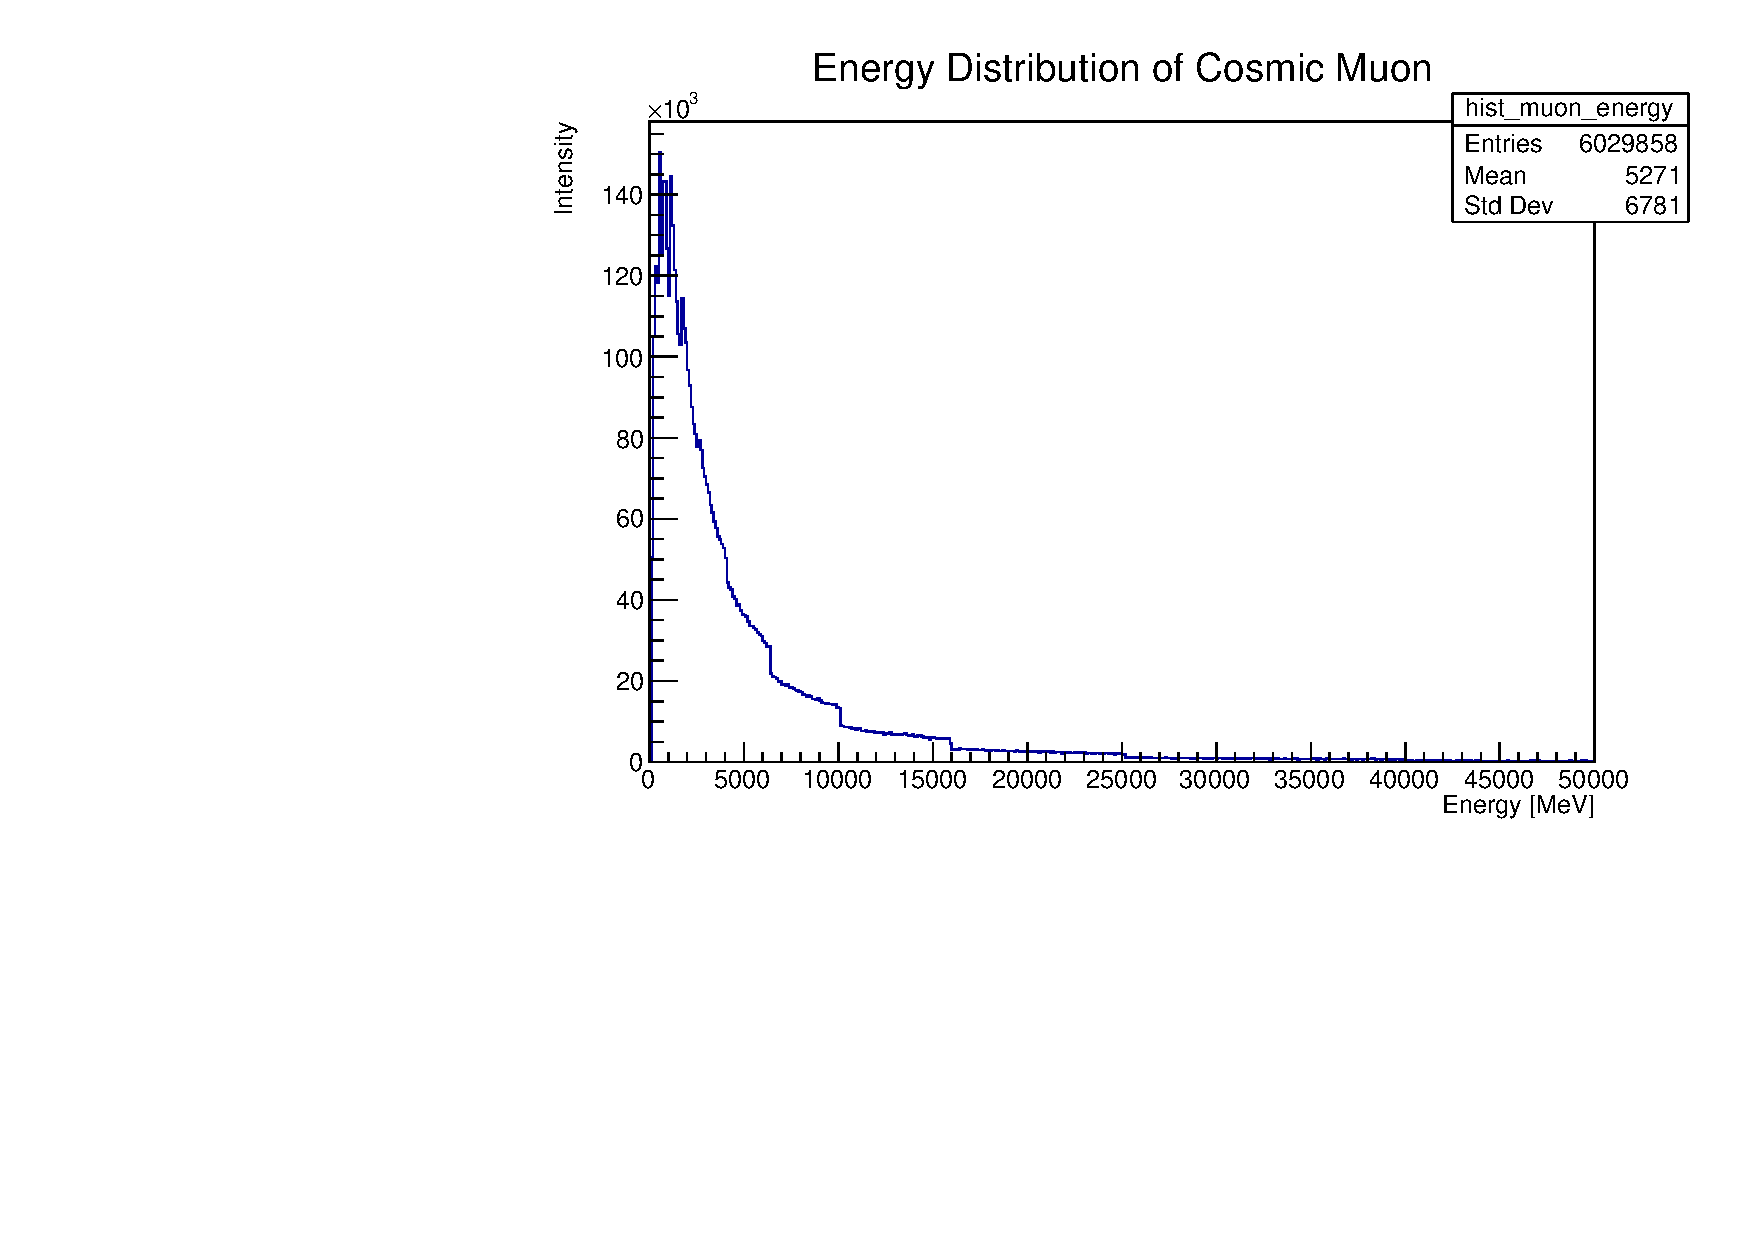
\includegraphics[height=5cm]{img/muon_energy_distribution.pdf}
        \caption{CRYによって生成した$\mu$粒子のエネルギー分布}
        \label{fig:muon_energy_distribution}
    \end{minipage}
    \begin{minipage}[b]{0.47\linewidth}
        \centering
        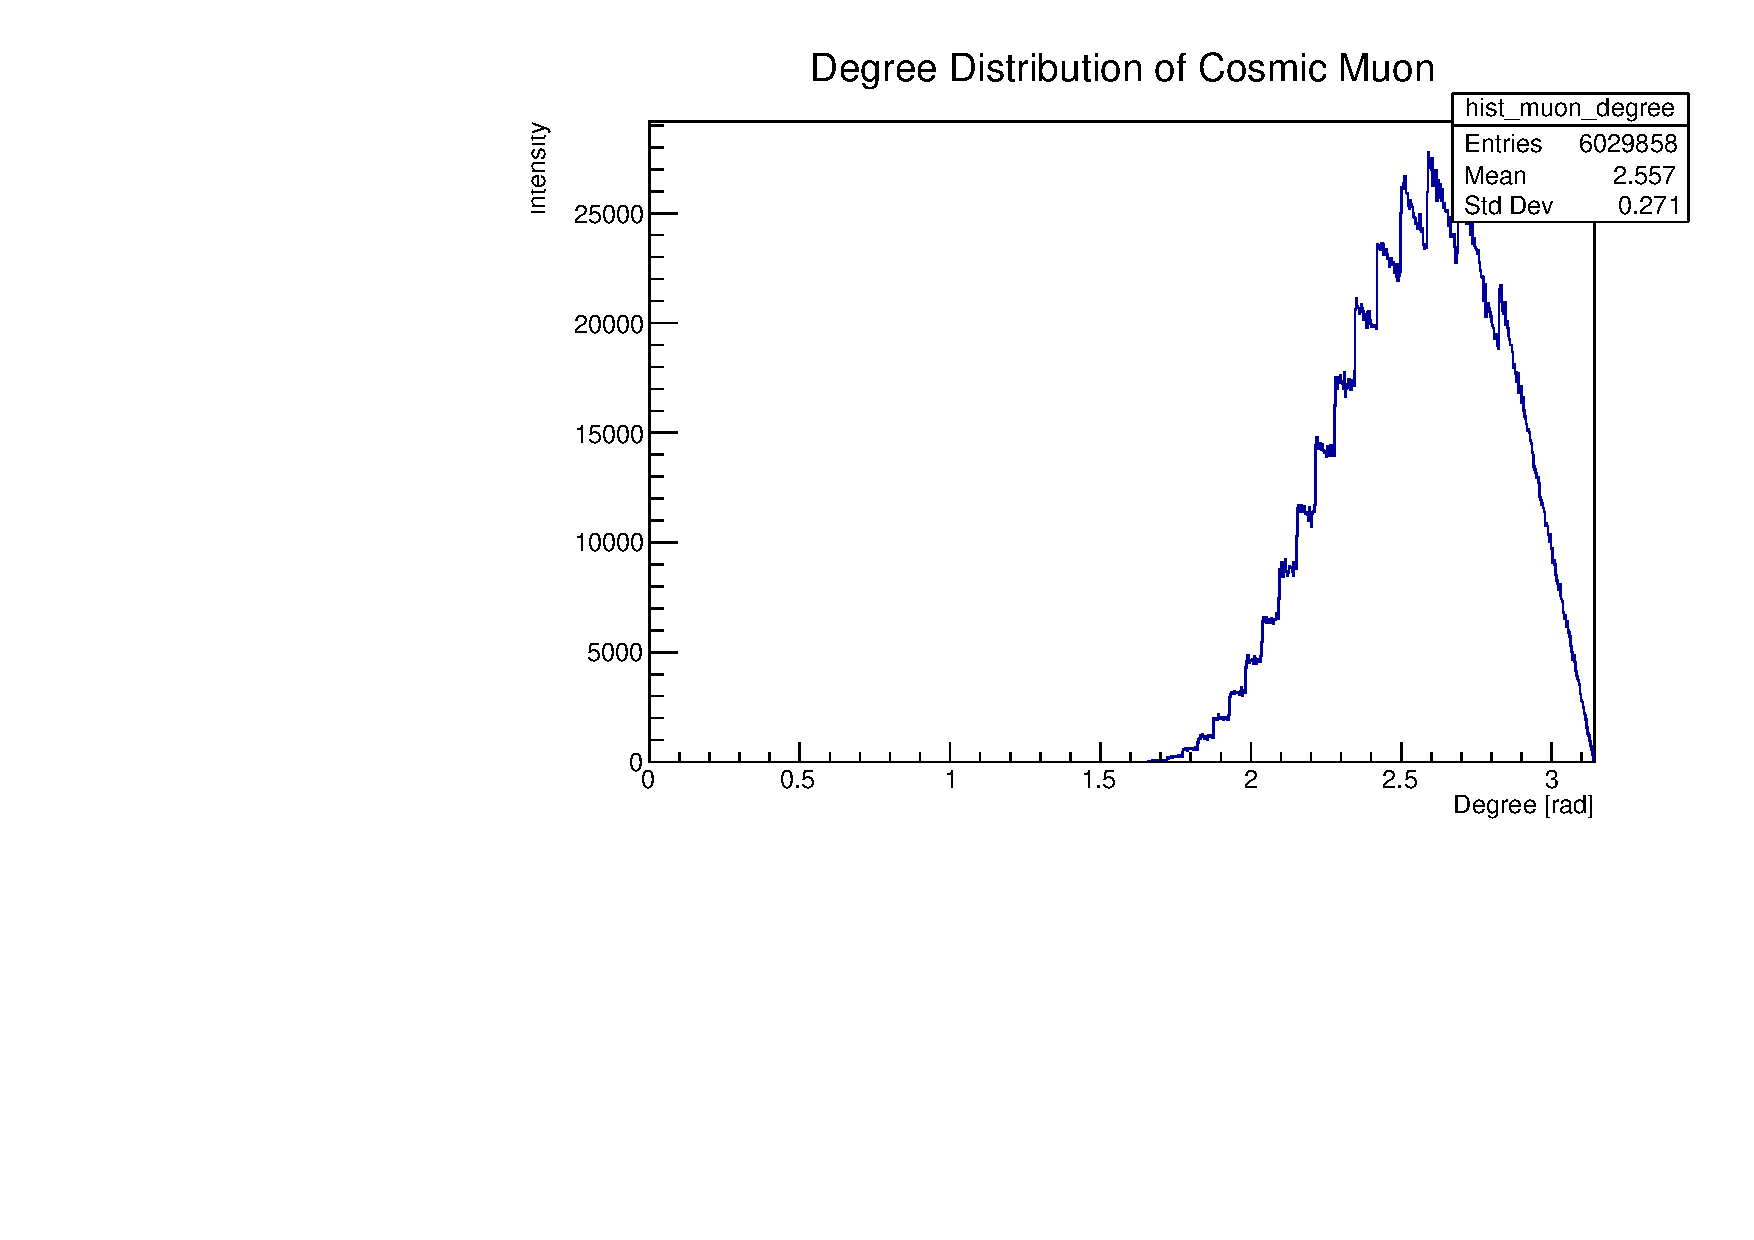
\includegraphics[height=5cm]{img/muon_degree_distribution.pdf}
        \caption{CRYによって生成した$\mu$粒子の角度分布}
        \label{fig:muon_degree_distribution}
    \end{minipage}
\end{figure}
図\ref{fig:muon_energy_distribution}より、入射$\mu$粒子は2000MeVあたりのエネルギーを持ったものが多いがそれよりも高エネルギーな粒子も存在するということがわかる。
図\ref{fig:muon_degree_distribution}においてdegree 0 は$z$軸正の方向を指しているので分布より斜め下向きに入射している粒子が多いことがわかる。
また、ヒストグラムのエントリー数が約600万イベントであることよりトリガーシンチレータを通過してもすべての粒子が検出器に入射するわけではないということがわかる。

今回シミュレーションを行った目的としては, 検出器内での光生成反応がどれくらいの割合で発生するのか求めることである.

\section{シミュレーション結果}
今回のシミュレーションにおいては光生成反応として入射$\mu$粒子からパイオンが発生したイベントを選んだ.

一番下のシンチレータまで$\mu$粒子が到達したイベントは全イベントのうち1,937,095イベントで効率は0.194であった.
また, シンチレータ内で反応して$\pi$が出たイベントは19イベントで効率は$1.90 \times10^{-6}$であった.
実際の測定器に$\mu$粒子が入射するレートは15count/secであったので, 1秒に$2.85 \times10^{-5}$だけ$\pi$が出てくるイベントがあるということになる.
実際約260時間測定を行ったので$1.2 \times10^{7}$万イベント得られた.
このことより, 今回用いた検出器においても光生成反応が起きて$\pi$が出てくるイベントというのが数十イベントくらいは観測できそうだということがわかった.

\begin{table}[H]
    \centering
    \caption{シミュレーションによるデータ}
    \label{tab:simu_data}
    \begin{tabular}{|c|r|}
        \hline
        総イベント                               & 10,000,000 \\ \hline
        1番下の層まで$\mu$粒子が通過したイベント & 1,937,095  \\ \hline
        $\pi$が出たイベント                      & 19         \\ \hline
    \end{tabular}
\end{table}

下の図\ref{fig:simu_track},\ref{fig:simu_pixel}は, 後述(\ref{sec:anal:eventcut}節)する解析プログラムを用いてシミュレーションデータを解析した図である.
このイベントだと宇宙線$\mu$粒子が検出器内で反応して2粒子出たことがわかる.それぞれの粒子の失ったエネルギーをシミュレーション結果から計算するとどの粒子か特定することができる。
\begin{figure}[H]
    \begin{minipage}[b]{0.47\linewidth}
        \centering
        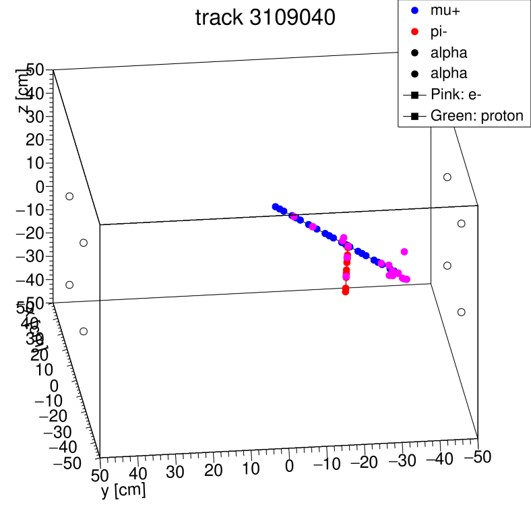
\includegraphics[height=5cm]{img/track_pion.jpg}
        \caption{検出器内でのトラックの様子}
        \label{fig:simu_track}
    \end{minipage}[b]
    \begin{minipage}[b]{0.47\linewidth}
        \centering
        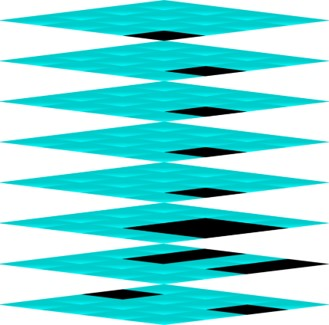
\includegraphics[height=5cm]{img/track_simulation.jpg}
        \caption{各シンチレータの鳴ったピクセル}
        \label{fig:simu_pixel}
    \end{minipage}
\end{figure}

